\documentclass[]{article}
\usepackage{lmodern}
\usepackage{amssymb,amsmath}
\usepackage{ifxetex,ifluatex}
\usepackage{fixltx2e} % provides \textsubscript
\ifnum 0\ifxetex 1\fi\ifluatex 1\fi=0 % if pdftex
  \usepackage[T1]{fontenc}
  \usepackage[utf8]{inputenc}
\else % if luatex or xelatex
  \ifxetex
    \usepackage{mathspec}
  \else
    \usepackage{fontspec}
  \fi
  \defaultfontfeatures{Ligatures=TeX,Scale=MatchLowercase}
\fi
% use upquote if available, for straight quotes in verbatim environments
\IfFileExists{upquote.sty}{\usepackage{upquote}}{}
% use microtype if available
\IfFileExists{microtype.sty}{%
\usepackage{microtype}
\UseMicrotypeSet[protrusion]{basicmath} % disable protrusion for tt fonts
}{}
\usepackage[margin=1in]{geometry}
\usepackage{hyperref}
\hypersetup{unicode=true,
            pdftitle={Displacement of fishing effort by Large Scale Marine Protected Areas},
            pdfborder={0 0 0},
            breaklinks=true}
\urlstyle{same}  % don't use monospace font for urls
\usepackage{natbib}
\bibliographystyle{nature}
\usepackage{longtable,booktabs}
\usepackage{graphicx,grffile}
\makeatletter
\def\maxwidth{\ifdim\Gin@nat@width>\linewidth\linewidth\else\Gin@nat@width\fi}
\def\maxheight{\ifdim\Gin@nat@height>\textheight\textheight\else\Gin@nat@height\fi}
\makeatother
% Scale images if necessary, so that they will not overflow the page
% margins by default, and it is still possible to overwrite the defaults
% using explicit options in \includegraphics[width, height, ...]{}
\setkeys{Gin}{width=\maxwidth,height=\maxheight,keepaspectratio}
\IfFileExists{parskip.sty}{%
\usepackage{parskip}
}{% else
\setlength{\parindent}{0pt}
\setlength{\parskip}{6pt plus 2pt minus 1pt}
}
\setlength{\emergencystretch}{3em}  % prevent overfull lines
\providecommand{\tightlist}{%
  \setlength{\itemsep}{0pt}\setlength{\parskip}{0pt}}
\setcounter{secnumdepth}{0}
% Redefines (sub)paragraphs to behave more like sections
\ifx\paragraph\undefined\else
\let\oldparagraph\paragraph
\renewcommand{\paragraph}[1]{\oldparagraph{#1}\mbox{}}
\fi
\ifx\subparagraph\undefined\else
\let\oldsubparagraph\subparagraph
\renewcommand{\subparagraph}[1]{\oldsubparagraph{#1}\mbox{}}
\fi

%%% Use protect on footnotes to avoid problems with footnotes in titles
\let\rmarkdownfootnote\footnote%
\def\footnote{\protect\rmarkdownfootnote}

%%% Change title format to be more compact
\usepackage{titling}

% Create subtitle command for use in maketitle
\newcommand{\subtitle}[1]{
  \posttitle{
    \begin{center}\large#1\end{center}
    }
}

\setlength{\droptitle}{-2em}

  \title{Displacement of fishing effort by Large Scale Marine Protected Areas}
    \pretitle{\vspace{\droptitle}\centering\huge}
  \posttitle{\par}
  \subtitle{Updated on 2018-09-27}
  \author{Juan Carlos Villaseñor-Derbez\textsuperscript{1} John
Lynham\textsuperscript{2}}
    \preauthor{\centering\large\emph}
  \postauthor{\par}
      \predate{\centering\large\emph}
  \postdate{\par}
    \date{\textsuperscript{1}Bren School of Environmental Science and Management,
University of California Santa Barbara, Santa Barbara, CA
\textsuperscript{2}Department of Economics, University of Hawaii at
Manoa, Honolulu, HI}

\usepackage{float}
\floatplacement{figure,table}{H}
\usepackage{lineno}
\linenumbers

\begin{document}
\maketitle
\begin{abstract}
Large-scale Marine Protected Areas (LSMPAs) have seen a significant
increase over the last years. Fishing effort is effectively eliminated
within these protected areas upon implementation. The benefits of
reducing effort have been largely studied, and include increases in
abundance, biomass, and diversity within the bounded regions. These
no-take zones may produce spillover effects, which provide fish for
outside areas. However, the economic and ecological implications of
displacing fishing effort are not yet fully understood. Novel data
products that track fishing effort at the vessel-level allow us to
identify changes in fleet- and vessel-level behavior upon the
implementation of protected areas, as well as how these redistribute.
This papers evaluates the implications of implementing LSMPA, by
evaluating changes in fishing hours, showing that vessels in the
effected region reduce fishing effort after the implementation of PIPA.
Our results are robust to a set of specifications. We also track the
relative spatial allocation of fishing events thorugh time, and identify
that areas closer to PIPA show an increase in relative fishing hourse
due to the displacement of PIPA-fishing vessels. Our results not only
provide an impact evaluation of the effect of LSMPAs on fishing
activity, but provide insights into vessel redistribution dynamics,
which may have ecological and economic implications.
\end{abstract}

{
\setcounter{tocdepth}{4}
\tableofcontents
}
\clearpage

\section{Introduction}\label{introduction}

This work identifies the behavioral changes of fishing vessels due to
the implementation of PIPA. Not only can we identify temporal changes in
fishing patterns (\emph{i.e.} time and distance), but also spatial
patterns. Our vessel-level tracks allow us to see where PIPA-fishing
vessels go after the closure, providing empirical insights about the
redistribution of fishing effort after the implementaion of a MPA.

\section{Methods}\label{methods}

This section is divided into two main parts. First, we provide a general
description of AIS data and the process of identification of
vessel-level events done by Global Fishing Watch \footnote{\href{globalfishingwatch.org}{Global
  Fishing Watch}}. Alongside, we describe the subset of data that we use
for these analyses. When relevant, we also point out possible
shortcommings in the data, or factors that must be considered in the
later analyses. Then we move on to explain our identification strategy,
and the main analyses that we undertake.

\subsection{Data}\label{data}

\subsubsection{AIS data}\label{ais-data}

Automatic Identification Systems are on-board devices intended to
provide at-sea saftey and prevent ship collisions by broadcasting vessel
locations to surrounding vessels. These broadcasted positions can be
recorded by satellites and land-based antenas. GFW uses a neural network
to infer vessel characteristics and whether each broadcasted position
represents a fishing event, thus allowing us to estimate near real-time
fishing events globally \citep{kroodsma_2018}. The recent addition of
satellites that can receive AIS signals causes an apparent increase in
the number of broadcasted AIS messages (\emph{i.e.} points) and
therefore fishing hours. It is therefore important to be cautious when
comparing temporal trends. The variability in AIS data and dynamic ocean
conditions require that temporal trends be taken into account. We do
that by incorporating a series of controls, which are defined in the
following section.

\subsubsection{PIPA data}\label{pipa-data}

The GFW data contain 233 purse seiners and longliners that have fished
within PIPA waters. From these, only 217 did so at least once before
2015, but only 183 continued to fish after 2015\footnote{The 34 missing
  vessels might have exited the fishery, been decomissioned or sold
  (therefore chaning their AIS and mmsi), or turned off their AIS
  transmiters. On either case, we are not able to observe these.}.
Vessels that fished within PIPA before implementation might stop fishing
afterwards, therefore not being observable in the post-treatment period.
New vessels might have also entered the fishery after PIPA closure, and
were likely not exposed to the policy intervention in the pre-treatment
period. Therefore, we define our treatment and control groups as
follows. The treatment group contains all vessels that fished within
PIPA at least once before the closure, and that continued to fish
elsewhere afterwards. The control group has vessels that never fished
within PIPA waters, belong to other PNA countries, and have fished in
surrounding areas (\emph{i.e.} PNA-countries' EEZ) before and after PIPA
closure. Figure \ref{fig:baci_strict} provides a visual representation
of the vessel-level that make up each of group through time.

Tables \ref{tab:baci_n}, \ref{tab:baci_n_s}, and \ref{tab:baci_h} show
the number of vessels, number of vessels following a BACI design, and
fishing hours, respectively. Tables show data grouped by gear
(longlines, purse seines), group (treated, control), and period (before,
after). The relative change (After / Before) is also shown. Table
\ref{tab:baci_n} shows information for all fishing vessels in the
dataset, while Tables \ref{tab:baci_n_s} and \ref{tab:baci_h} show
information for vessels that meet the BACI design (i.e.~excludes vessels
that only appear at one point in time).

\begin{figure}
\centering
\includegraphics{../img/BACI_strict_gear.png}
\caption{\label{fig:baci_strict}Stream of fishing events by vessels
(stacked on the y-axis due to space) through time (x-axis). Each dot
represent a vessel-month, with colors indicating the pre and post
periods, and pannels separating between gear and treated or control
groups.}
\end{figure}

\begin{table}[H]

\caption{\label{tab:unnamed-chunk-4}\label{tab:baci_n}Number of fishing vessels (identified by mmsi) for each gear before and after PIPA implementation.}
\centering
\begin{tabular}[t]{llrrr}
\toprule
Gear & Treatment & Before & After & Change (A / B)\\
\midrule
drifting\_longlines & FALSE & 105 & 218 & 2.0761905\\
drifting\_longlines & TRUE & 139 & 118 & 0.8489209\\
purse\_seines & FALSE & 49 & 89 & 1.8163265\\
purse\_seines & TRUE & 78 & 81 & 1.0384615\\
\bottomrule
\end{tabular}
\end{table}

\begin{table}[H]

\caption{\label{tab:unnamed-chunk-5}\label{tab:baci_n_s}Number of fishing vessels (identified by mmsi) for each gear before and after PIPA implementation.}
\centering
\begin{tabular}[t]{llrrr}
\toprule
Gear & Treatment & Before & After & Change (A / B)\\
\midrule
drifting\_longlines & FALSE & 88 & 88 & 1\\
drifting\_longlines & TRUE & 115 & 115 & 1\\
purse\_seines & FALSE & 38 & 38 & 1\\
purse\_seines & TRUE & 68 & 68 & 1\\
\bottomrule
\end{tabular}
\end{table}

\begin{table}[H]

\caption{\label{tab:unnamed-chunk-6}\label{tab:baci_h}Mean fishing hours for each gear before and after}
\centering
\begin{tabular}[t]{llrrr}
\toprule
Gear & Treatment & Before & After & Change (A / B)\\
\midrule
drifting\_longlines & FALSE & 481.42502 & 473.5823 & 0.9837094\\
drifting\_longlines & TRUE & 548.22580 & 524.8121 & 0.9572919\\
purse\_seines & FALSE & 66.50483 & 172.3775 & 2.5919548\\
purse\_seines & TRUE & 56.87322 & 146.2015 & 2.5706563\\
\bottomrule
\end{tabular}
\end{table}

\subsection{Analysis}\label{analysis}

\subsubsection{Change in behavior}\label{change-in-behavior}

The first analysis focuses on identifying the response of fishing
vessels to PIPA closure. Our variables of interests are fishing effort,
indicated by total fishing hours per month, and distance traveled (Km)
on every fishing trip. We compare fishing hours\footnote{And soon,
  distance} before and after the implementation of PIPA using a
Difference-in-Differences approach, where we track the variable of
interest for vessels that used to fish inside PIPA and vessels that
never fished inside PIPA, before and after PIPA implementation. Our
specification is the following:

\[
y_{i,t} = \alpha + \beta_1 Post_t + \beta_2 Treat_i + \beta_3 Post_t \times Treat_i + \mu_t + \phi_t + \gamma_i + \epsilon_{i,t}
\]

Where \(y_{ijkl}\) is the variable of interest for vessel \(i\) in time
period \(t\). A dummy variable \(Post_i\) takes the value of 0 for all
dates prior to PIPA implementation and a value of 1 por all dates
including and following PIPA implementation. \(Treat_i\) is a dummy
variable indicating whether a vessel belongs to the control
(\(Treat_i = 0\)) or treatment (\(Treat_i = 1\)) group. \(\alpha\) is
the standard intercept, \(\beta_1\) captures the \emph{ex post} change,
\(\beta_2\) captures the difference between treated and control groups,
and \(\beta_3\) is our parameter of interest: de DiD estimate capturing
the treatment effect. Finally, \(\mu_t\), \(\phi_t\), and \(\gamma_i\)
represent month-, year-, and flag-level dummies that account for
seasonality or country-level management interventions.

\subsubsection{Vessel displacement and
redistribution}\label{vessel-displacement-and-redistribution}

Our second part of the analyses focuses on the redistribution of fishing
effort. In other words, identifying where do vessels that used to fish
inside PIPA go after its establishment. We calculate the monthly
relative distribution of fishing hours by all treated vessels across all
fished EEZs and the high seas. These trends are shown in Figure
\ref{fig:redist_trend}. EEZs that had sproadic fishing events were
pooled into a group of ``others'', leaving us with a total of n = 12
spatially defined regions (\emph{i.e.} EEZs, High Seas, ``other EEZs'').
Figure \ref{fig:redist_trend_spa} shows the yearly average of the
relative spatial allocation of fishing efforts; this is the spatial
representation of \ref{fig:redist_trend} averaged by year.

\begin{figure}
\centering
\includegraphics{C:/Users/JC/Documents/GitHub/MPA_displacement/docs/Manuscript_files/figure-latex/unnamed-chunk-9-1.pdf}
\caption{\label{fig:unnamed-chunk-9}\label{fig:redist_trend}}
\end{figure}

To evaluate this change in effort allocation, we regress our variable of
interest, fishing hours, on the interaction between a dummy variable
indicating the policy intervention and a dummy variable for countries,
to obtain the by-country change in proportional allocation of fishing
effort:

\[
y_{i,t} = \alpha + \beta_1Post_t + \beta_2Country_i + \beta3Post_t \times Country_i + \epsilon_{i,t}
\]

Our variable of interest, \(y_{i,t}\) represents the proportion of
fishing hours that country \(i\) receives at time \(t\). \(Post\) also
represents a policy dummy that takes the value of 0 for all dates before
implementation of PIPA, and 1 otherwise. \(Country\) is a dummy variable
for countries, interpreted as individual EEZs, the high seas, and a
group of ``other EEZs''. Our parameter of interest is \(\beta_3\), which
captures the country-level change in proportional fishing effort.

\section{Results}\label{results}

Fig. \ref{fig:all_vessels} shows that mean fishing hours for purse
seiners have an abrupt increase, just before January 1st, 2015. This
trend is observed for both treated and control groups. Longliners,
however, show a more stable trend. The number of mmsi codes increases
through time. This can largel be explained by the addition of more
satellits, which increasedetectability of vessels. As expected total
fishing hours follow a similar trend to that of mmsi numbers. Results of
the regressions for each gear type are shown in Tables \ref{tab:purse}
and \ref{tab:long}. Column (1) presents the DiD regression with no fixed
effects, column (2) includes month fixed effects, column (3) includes
month and year fixed effects, and column (4) includes month, year, and
flag fixed effects. Figures \ref{fig:puse} and \ref{fig:long} represent
the same coefficient estimates.

\begin{figure}
\centering
\includegraphics{C:/Users/JC/Documents/GitHub/MPA_displacement/docs/Manuscript_files/figure-latex/unnamed-chunk-11-1.pdf}
\caption{\label{fig:unnamed-chunk-11}\label{fig:all_vessels}Fishing hours
and number of vessels by month for all vessels. Vertical dashed line
indicates PIPA closure.}
\end{figure}

\clearpage

\subsection{Change in behavior}\label{change-in-behavior-1}

\subsubsection{Purse seiners}\label{purse-seiners}

\begin{table}[!htbp] \centering 
  \caption{\label{tab:purse}Fishing hours from GFW for purse seiners (n = 106; 38 control, 68 treatment). Asterisks indicate significance levels. Numbers in parenthesis represent heteroskedastic-robuste standard errors.} 
  \label{} 
\begin{tabular}{@{\extracolsep{5pt}}lcccc} 
\\[-1.8ex]\hline 
\hline \\[-1.8ex] 
 & \multicolumn{4}{c}{\textit{Dependent variable:}} \\ 
\cline{2-5} 
\\[-1.8ex] & \multicolumn{4}{c}{hours} \\ 
\\[-1.8ex] & (1) & (2) & (3) & (4)\\ 
\hline \\[-1.8ex] 
 post & 105.873$^{***}$ & 107.859$^{***}$ & 113.466$^{***}$ & 102.890$^{***}$ \\ 
  & (5.532) & (5.364) & (5.887) & (6.076) \\ 
  & & & & \\ 
 treated & $-$9.632$^{**}$ & $-$8.924$^{**}$ & $-$8.334$^{**}$ & $-$3.076 \\ 
  & (4.257) & (4.023) & (3.725) & (4.540) \\ 
  & & & & \\ 
 post:treated & $-$16.544$^{**}$ & $-$16.889$^{***}$ & $-$17.235$^{***}$ & $-$11.150$^{*}$ \\ 
  & (6.481) & (6.358) & (6.126) & (6.162) \\ 
  & & & & \\ 
 Constant & 66.505$^{***}$ & 61.758$^{***}$ & 40.085$^{***}$ & 61.569$^{***}$ \\ 
  & (3.780) & (5.352) & (5.699) & (9.753) \\ 
  & & & & \\ 
\hline \\[-1.8ex] 
Month FE & No & Yes & Yes & Yes \\ 
Year FE & No & No & Yes & Yes \\ 
Flag FE & No & No & No & Yes \\ 
Observations & 3,692 & 3,692 & 3,692 & 3,692 \\ 
R$^{2}$ & 0.238 & 0.262 & 0.312 & 0.339 \\ 
\hline 
\hline \\[-1.8ex] 
\textit{Note:}  & \multicolumn{4}{r}{$^{*}$p$<$0.1; $^{**}$p$<$0.05; $^{***}$p$<$0.01} \\ 
\end{tabular} 
\end{table}

\begin{figure}
\centering
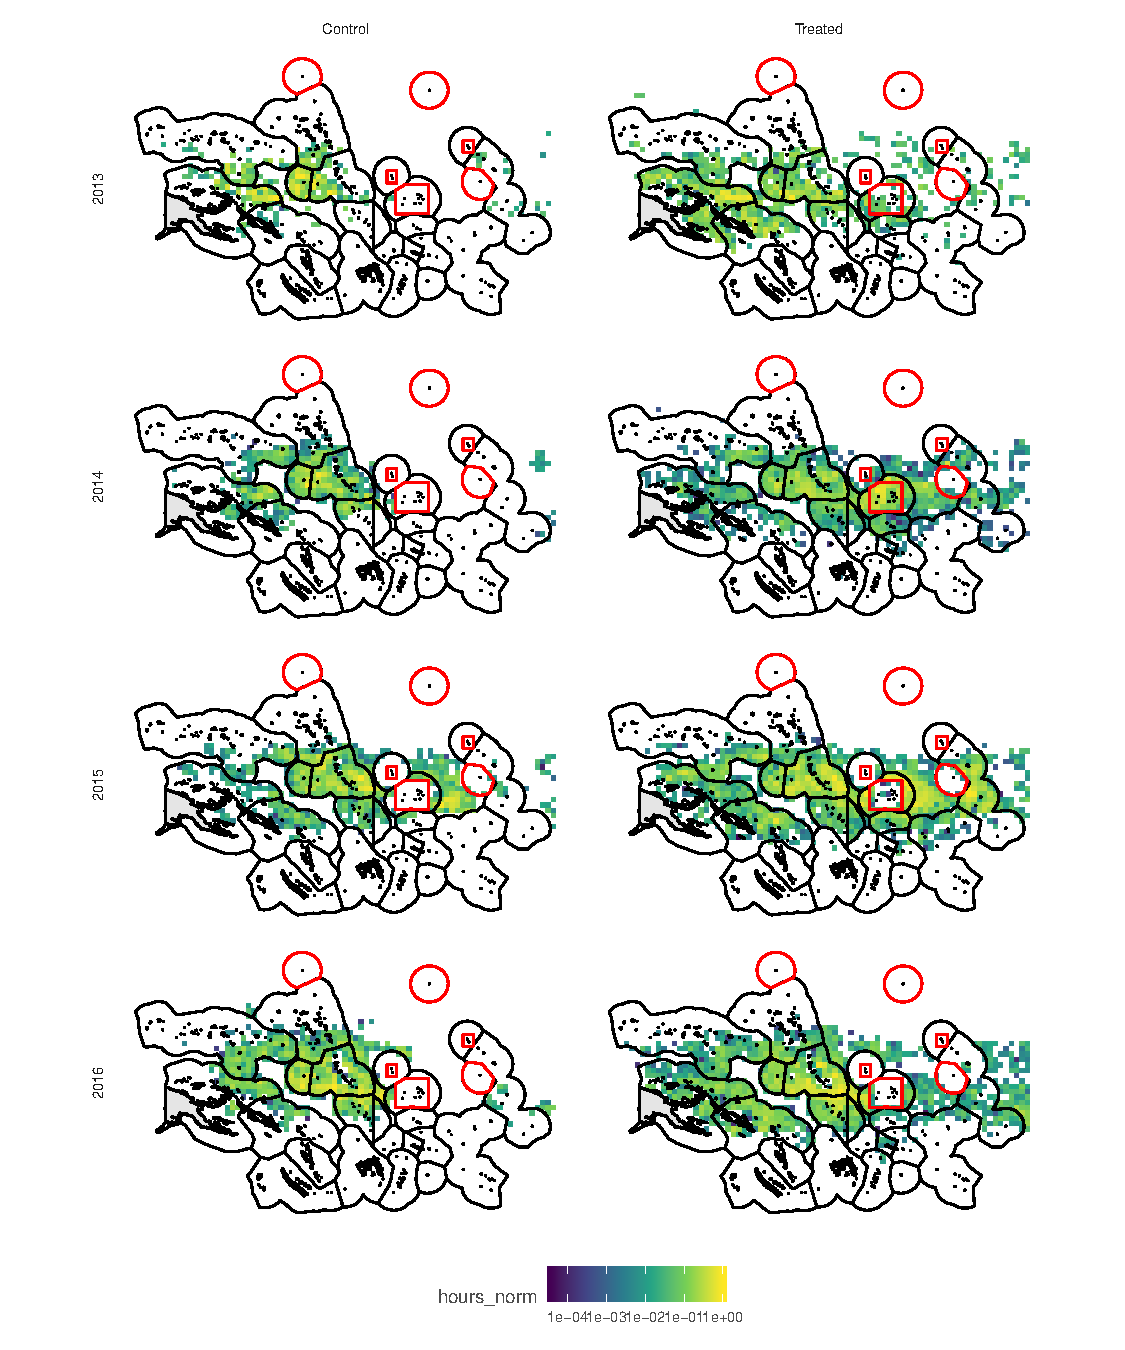
\includegraphics{C:/Users/JC/Documents/GitHub/MPA_displacement/docs/Manuscript_files/figure-latex/unnamed-chunk-13-1.pdf}
\caption{\label{fig:unnamed-chunk-13}\label{fig:puse}Coefficient estimates
for each model. Top pannel indicates variable, x-axis represents model
specification, and y-axis coefficient estimate.}
\end{figure}

\clearpage

\subsubsection{Longliners}\label{longliners}

\begin{table}[!htbp] \centering 
  \caption{\label{tab:long}Fishing hours from GFW for longliners (n = 203; 88 control, 115 treatment).. Asterisks indicate significance levels. Numbers in parenthesis represent heteroskedastic-robuste standard errors.} 
  \label{} 
\begin{tabular}{@{\extracolsep{5pt}}lcccc} 
\\[-1.8ex]\hline 
\hline \\[-1.8ex] 
 & \multicolumn{4}{c}{\textit{Dependent variable:}} \\ 
\cline{2-5} 
\\[-1.8ex] & \multicolumn{4}{c}{hours} \\ 
\\[-1.8ex] & (1) & (2) & (3) & (4)\\ 
\hline \\[-1.8ex] 
 post & $-$7.843 & $-$4.894 & $-$7.580 & 24.708$^{***}$ \\ 
  & (7.514) & (7.480) & (9.336) & (9.315) \\ 
  & & & & \\ 
 treated & 66.801$^{***}$ & 69.434$^{***}$ & 69.959$^{***}$ & 18.878$^{***}$ \\ 
  & (6.541) & (6.549) & (6.603) & (7.257) \\ 
  & & & & \\ 
 post:treated & $-$15.571$^{*}$ & $-$17.806$^{**}$ & $-$18.340$^{**}$ & $-$25.775$^{***}$ \\ 
  & (8.958) & (8.899) & (8.936) & (8.743) \\ 
  & & & & \\ 
 Constant & 481.425$^{***}$ & 450.475$^{***}$ & 447.866$^{***}$ & 430.947$^{***}$ \\ 
  & (5.733) & (9.239) & (10.280) & (24.476) \\ 
  & & & & \\ 
\hline \\[-1.8ex] 
Month FE & No & Yes & Yes & Yes \\ 
Year FE & No & No & Yes & Yes \\ 
Flag FE & No & No & No & Yes \\ 
Observations & 8,558 & 8,558 & 8,558 & 8,558 \\ 
R$^{2}$ & 0.026 & 0.044 & 0.044 & 0.107 \\ 
\hline 
\hline \\[-1.8ex] 
\textit{Note:}  & \multicolumn{4}{r}{$^{*}$p$<$0.1; $^{**}$p$<$0.05; $^{***}$p$<$0.01} \\ 
\end{tabular} 
\end{table}

\begin{figure}
\centering
\includegraphics{C:/Users/JC/Documents/GitHub/MPA_displacement/docs/Manuscript_files/figure-latex/unnamed-chunk-15-1.pdf}
\caption{\label{fig:unnamed-chunk-15}\label{fig:long}Coefficient estimates
for each model. Top pannel indicates variable, x-axis represents model
specification, and y-axis coefficient estimate.}
\end{figure}

\subsection{Effort displacement and
redistribution}\label{effort-displacement-and-redistribution}

\includegraphics{C:/Users/JC/Documents/GitHub/MPA_displacement/docs/Manuscript_files/figure-latex/unnamed-chunk-16-1.pdf}

\renewcommand\refname{References}
\bibliography{references.bib}


\end{document}
